\chapter{Programming and Proving in Cubical Agda}
Agda \cite{norellDependentlyTypedProgramming2008} is a dependently-typed, pure,
functional programming language and proof assistant.
In this thesis, we will use it to explore and prove things about finite and
countable types.
Along the way, we will learn about proofs in a dependent setting, functional
programming, and Homotopy Type Theory.

In this chapter we will introduce the language with some basic examples, and
explain a little about how to program and prove in Agda.
Some Haskell knowledge will help, as much of the syntax (any many concepts) are
similar, but it is possible to struggle through without it.
It is recommended to try out the code examples in your own editor, or to look at
them in the real Agda files in the source.
\todo{Set this up: organise code examples better?}

\section{Basic Functional Programming in Agda}
The basic unit of functionality in Agda is the \emph{type}.
Let's define a type: the type of booleans (we include the equivalent code in
Haskell on the right).
\begin{agdalisting} \label{bool-def}
  \begin{multicols}{2} \centering
    \ExecuteMetaData[agda/Snippets/Bool.tex]{bool-def} \columnbreak
    \ExecuteMetaData[haskell/Bool.tex]{bool-def}
  \end{multicols}\vspace{-2\baselineskip}
\end{agdalisting}
There's a lot of syntax wrapped up in this small snippet.
In prose, it provides four basic pieces of information:
\begin{enumerate}
  \item We are defining a new \AgdaKeyword{data} type.
  \item Its name is \AgdaDatatype{Bool}.
  \item \AgdaDatatype{Bool} is a \AgdaFunction{\(\text{Type}_0\)} kind of thing.
  \item There are two ways to construct values of type \AgdaDatatype{Bool}:
    \AgdaInductiveConstructor{false} and \AgdaInductiveConstructor{true}.
\end{enumerate}
Let's explain each piece one by one.

The last point is the simplest: we have listed the ways to construct values of
type \AgdaDatatype{Bool}.
Two ways, in fact, \AgdaInductiveConstructor{true} and
\AgdaInductiveConstructor{false}, and they're called the constructors.
We can use these constructors in programs by (for instance) assigning them to
variables.
\begin{multicols}{2}\centering
  \ExecuteMetaData[agda/Snippets/Bool.tex]{bool-val}\columnbreak
  \ExecuteMetaData[haskell/Bool.tex]{bool-val}
\end{multicols}\vspace{-2\baselineskip}\noindent
Here we've declared a variable\footnotemark\;called \AgdaFunction{a-boolean} with
the type \AgdaDatatype{Bool}, and said it is equal to the value
\AgdaInductiveConstructor{true}.

\footnotetext{Note that although we use the term ``variable'', the value of the
  variable \AgdaFunction{a-boolean} can not change.
  We couldn't reassign it on the following line.}

Now back to the first point: we say that we're defining a new \AgdaKeyword{data}
type.
Using the ``\AgdaKeyword{data}'' keyword is just one of the many ways of
defining types: it basically means that we are going to define the type by
listing all of its constructors.
Another way to define types is with \AgdaKeyword{record}, which we'll see later,
and yet another way is to define a type by referring to other already-defined types.
Here, for instance, we can define the type \AgdaFunction{Boolean}:
\begin{agdalisting*}
  \ExecuteMetaData[agda/Snippets/Bool.tex]{boolean}
\end{agdalisting*}
This snippet says ``I am defining a new thing called \AgdaFunction{Boolean}, it
is a \AgdaFunction{\(\text{Type}_0\)}, and it is equal to \AgdaDatatype{Bool}''.
Of course this isn't a very interesting declaration: as the equals sign implies,
\AgdaFunction{Boolean} is the same as \AgdaFunction{Bool} (other than the
spelling).
We've basically defined a synonym for the old type.

The third point is the most interesting: we say that \AgdaDatatype{Bool} is a
``\AgdaFunction{\(\text{Type}_0\)}'' kind of thing.
What does this mean?

Well, we've seen that we can assign types to variables just as easily as we
might assign values to variables: this is what was happening in the
\AgdaFunction{Boolean} example.
In fact, in Agda, there is no real distinction between ``types'' and ``values'':
types like \AgdaDatatype{Bool} \emph{are} values, just as much as
\AgdaInductiveConstructor{true} or \AgdaInductiveConstructor{false}!
This means that our types must themselves have types: hence we say that
\AgdaFunction{Boolean} has type \AgdaFunction{\(\text{Type}_0\)}.

But why the subscript 0?
Well we know that types are values in Agda, and so they themselves have types.
We know that the type of \AgdaDatatype{Bool} is
\AgdaFunction{\(\text{Type}_0\)}.
But what's the type of \AgdaFunction{\(\text{Type}_0\)}?
It turns out that if we say:
\begin{agdalisting*}
  \(\AgdaFunction{\(\text{Type}_0\)} :  \AgdaFunction{\(\text{Type}_0\)}\)
\end{agdalisting*}
We actually introduce a paradox into the language: Girard's paradox
\cite{girardInterpretationFonctionelleElimination1972}.
This is the type-theoretic analogue of Russell's paradox, and, if present, it
would allow us to prove things that are not true.
So we disallow it.

Dependently-types programming languages have many different ways of resolving
the issue: Agda's approach is called \emph{universe polymorphism}.
Basically, we say that the type of \AgdaInductiveConstructor{true} is
\AgdaDatatype{Bool}, the type of \AgdaDatatype{Bool} is
\AgdaFunction{\(\text{Type}_0\)}, the type of \AgdaFunction{\(\text{Type}_0\)}
is \AgdaFunction{\(\text{Type}_1\)}, the type of \AgdaFunction{\(\text{Type}_1\)}
is \AgdaFunction{\(\text{Type}_2\)}, and so on.

To be honest, avoiding Girard's paradox is one of things that isn't done
especially well in dependently-typed languages: most approaches require quite a
bit of tedious busywork from the programmer, and it's quite rare that a
programmer would run into a genuine universe size issue that exposes a deep
logical impossibility (we will run into one of the few cases in this thesis).
Most of the time, managing universe levels amounts to bookkeeping.
For that reason, and also because the current system of universe polymorphism in
Agda is quite under flux and likely to be changed soon, we won't spend too much
time on the topic.
Every code example provided is as universe-polymorphic as possible, though.
\section{Some Functions}
That's quite a lot of information on how to define things in Agda: let's look a
little about how to do computation.
What we need is a function:
\begin{agdalisting*}
  \ExecuteMetaData[agda/Snippets/Bool.tex]{not-def}
\end{agdalisting*}
This function is defined by pattern-matching: when the clause on the
left-hand-side of the equals sign is seen, the right-hand-side is what's
computed.

For a more complex example, we're going to need a more complex type:
\begin{agdalisting}
  \ExecuteMetaData[agda/Snippets/Nat.tex]{nat-def}
\end{agdalisting}
This is the type of the natural numbers.
With \AgdaDatatype{Bool} (Equation~\ref{bool-def}) we were able to list all the
actual values in the type: doing so for the natural numbers would somewhat bloat
the page count of this thesis.
Instead, we list the two ways to construct natural numbers: first,
\AgdaInductiveConstructor{zero} is a natural number.
Next, if you have a natural number, its successor
(\AgdaInductiveConstructor{suc}) is a natural number.

Agda has special syntax for constructing natural numbers: we can write
\AgdaNumber{3} instead of
\(\AgdaInductiveConstructor{suc}\;(\AgdaInductiveConstructor{suc}\;(\AgdaInductiveConstructor{suc}\;\AgdaInductiveConstructor{zero}))\).

Here's a function on the natural numbers:
\begin{agdalisting} \label{sub-def}
  \ExecuteMetaData[agda/Snippets/Nat.tex]{sub-def}
\end{agdalisting}
We've defined subtraction.

Notice that this function is defined as an operator: for the function
declaration (the line with the type signature), we put underscores where we
expect the arguments to the operator to go.

In the introduction, we described Agda as a ``total'' programming language.
This means that if we give a function the type \(A \rightarrow B\), then we have
also \emph{proven} that, given an \(A\), it will produce a \(B\) (in finite
time).

Practically speaking, this means that Agda will perform some checks on our
code to ensure that every function is indeed total.
Our definition of subtraction above (Equation~\ref{sub-def}), for instance,
truncates to zero when there's arithmetic underflow.
In other words \(5 - 6 = 0\), according to our definition.
We could have removed the clause which allows for this:
\begin{agdalisting*}
  \ExecuteMetaData[agda/Snippets/Nat.tex]{bad-sub}
\end{agdalisting*}
But now the expression \(5 - 6\) is undefined.

The other major check that Agda will preform on our function definitions is for
\emph{termination} (or productivity, which we will see later).
This checks that no function we write accidentally contains an infinite loop.
Most of the time, we won't butt heads with the
termination checker, but it does happen occasionally, so it's helpful to
understand a little how it works. When we define the following function
(addition on the natural numbers):
\begin{agdalisting} \label{add-def}
  \ExecuteMetaData[agda/Snippets/Nat.tex]{add-def}
\end{agdalisting}
Agda checks that the argument to the recursive call is \emph{structurally
  smaller} than the argument given to the outer function.
``Structurally smaller'' effectively means that the smaller thing must be a
smaller structure contained entirely within the larger: in this case, \(n\) is
literally contained within the structure of the argument
\(\AgdaInductiveConstructor{suc}\;n\). \todo{express this better?}

Structural recursion is actually surprisingly powerful: a great many algorithms
can be converted to forms where the recursive calls recurse on some substructure
of their arguments.
It does require careful definitions, though.
For instance, the following will \emph{not} pass the termination checker:
\begin{agdalisting*}
  \ExecuteMetaData[agda/Snippets/Nat.tex]{bad-add}
\end{agdalisting*}
Though it defines the same function as Equation~\ref{add-def}, it doesn't make
it absolutely obvious to the termination checker that the first argument to the
recursive call (\(n - 1\)) is structurally smaller than the outer argument
(\(n\)).

Occasionally a function can't be refactored to the extent where it will be
obviously structurally terminating to Agda.
In those cases, there are facilities to describe more complex termination
conditions (although we should stress that these facilities are not
built in to the compiler or anything: they're actually just extremely clever
ways to express structural recursion), but if you have to reach for those
facilities it's usually a sign you've gone wrong.
We won't use them here.

One thing we haven't answered is \emph{why} we bother checking for termination
or totality.
The answer is that it's necessary for Agda to be a valid proof assistant.
Imagine if we could construct a type for ``proofs of the Riemann hypothesis''.
We might call it \AgdaFunction{RiemannIsTrue}.
In a language like Haskell, the following is a completely valid program:
\begin{agdalisting*}
  \ExecuteMetaData[agda/Snippets/Nat.tex]{riemann-proof}
\end{agdalisting*}
But of course we \emph{haven't} provided a proof of the Riemann hypothesis (and
if we had we certainly wouldn't have buried the lead to this extent).
The termination checker is vital to rule out these kinds of ``proofs'': that's
why it's an integral part of Agda.
\section{An Expression Evaluator}
Let's put all of the different things we've learned into a more complex example.
Later, we'll define a full solver for the Countdown problem
\cite{huttonCountdownProblem2002} \todo{find original cite for this}, at this
point we'll define a small part of it: the expression evaluator.

We want to define a language of arithmetic expressions.
With countdown in mind, we'll only need to support four operators, which we can
define in a simple data type:
\begin{agdalisting}
  \ExecuteMetaData[agda/Snippets/Expr.tex]{op-def}
\end{agdalisting}
Next, we'll define the actual type of expressions.
\begin{agdalisting}
  \ExecuteMetaData[agda/Snippets/Expr.tex]{expr-def}
\end{agdalisting}
What we've defined here is actually a simple leafy binary tree.
The syntax for the second constructor is not so simple, however: it defines a
\emph{mixfix} operator.
Each underscore in \AgdaInductiveConstructor{\(\_\langle \_ \rangle\_\)}
represents a hole which expressions can be put into.
This allows us to use the constructor like so:
\begin{agdalisting*}
  \ExecuteMetaData[agda/Snippets/Expr.tex]{example-expr}
\end{agdalisting*}

Evaluation of an expression is done by the following function:
\begin{agdalisting}
  \ExecuteMetaData[agda/Snippets/Expr.tex]{incorrect-eval}
\end{agdalisting}
We've introduced the \AgdaKeyword{with} syntax here: it functions somewhat like
a case expression in Haskell.
Basically, it allows us to pattern-match on the result of applying a function to
one of the input arguments without defining a new function.
\section{Safe Evaluation With Maybe}
The evaluator we have written isn't exactly correct.
It implies things like \(4 - 5 = 0\), or \(10 \div 3 = 3\), or \(2 \div 0 = 0\);
this doesn't make the function ``wrong'' per se, but it might be more desirable
to have expressions like \(2 \div 0\) be undefined.
It's especially important for countdown, as division by zero (or any of the
other equations) isn't permitted.

To remedy the problem we're going to introduce a new type.
\begin{agdalisting}
  \ExecuteMetaData[agda/Data/Maybe/Base.tex]{maybe-def}
\end{agdalisting}
\AgdaDatatype{Maybe} is a container that can contain at most one item.
It's the first \emph{parameterised} type we have seen: \AgdaDatatype{Maybe} can
contain an item of any type.
Here, for instance, is a \AgdaDatatype{Maybe} which contains the number 2:
\begin{agdalisting*}
  \ExecuteMetaData[agda/Snippets/Maybe.tex]{maybe-two}
\end{agdalisting*}
Or here is a \AgdaDatatype{Maybe} which doesn't contain anything, but whose type
says it could contain a function from \agdambb{N} to \agdambb{N}:
\begin{agdalisting*}
  \ExecuteMetaData[agda/Snippets/Maybe.tex]{maybe-nat-to-nat}
\end{agdalisting*}

Maybe is used often in functional programming to represent partiality: if you
have a function which is undefined for certain inputs, you can wrap
\AgdaDatatype{Maybe} around its return type, and return
\AgdaInductiveConstructor{nothing} for the cases where those inputs are given.
We can use it here, for instance, to define a version of subtraction which
doesn't truncate arithmetic underflow:
\begin{agdalisting}
  \ExecuteMetaData[agda/Snippets/Expr.tex]{safe-sub}
\end{agdalisting}
It's often also used for similar purposes as \verb+null+ is in imperative
programming, although it is of course far safer since it's impossible to forget
to check for \AgdaInductiveConstructor{nothing} by definition.

We can use \AgdaDatatype{Maybe} in our evaluator for expressions, so that we
return \AgdaInductiveConstructor{nothing} on expressions which evaluate to
undefined values.
That changes the type to the following:
\begin{agdalisting*}
  \ExecuteMetaData[agda/Snippets/Expr.tex]{eval-ty}
\end{agdalisting*}
The first case is relatively simple:
\begin{agdalisting*}
  \ExecuteMetaData[agda/Snippets/Expr.tex]{lit-case}
\end{agdalisting*}

The second two cases are slightly more complex: the result of evaluating each
sub-tree is \(\AgdaDatatype{Maybe}\;\agdambb{N}\), not \agdambb{N}, so we will
have to pattern-match on the outputs to check for
\AgdaInductiveConstructor{nothing}.
\begin{agdalisting*}
  \ExecuteMetaData[agda/Snippets/Expr.tex]{add-helper}
\end{agdalisting*}
Code like this is quite tedious.
Luckily, there's a common pattern we can abstract out: whenever we have a
multi-argument function, we can apply it to arguments wrapped in
\AgdaDatatype{Maybe} using the following two functions.
\begin{multicols}{2} \null \vfill
  \begin{agdalisting}
    \ExecuteMetaData[agda/Data/Maybe/Sugar.tex]{pure}
  \end{agdalisting} \vfill \null \columnbreak
  \begin{agdalisting}
    \ExecuteMetaData[agda/Data/Maybe/Sugar.tex]{ap}
  \end{agdalisting}
\end{multicols} \noindent
Any type which implements these functions (in a certain law-abiding way) is said
to be an ``Applicative Functor''
\cite{mcbrideApplicativeProgrammingEffects2008}, a full explanation of which is
beyond the scope of this thesis.

It might not be immediately clear how those two functions can help us.
Basically, we can replace the \AgdaFunction{add-helper} function with the
following:
\begin{agdalisting*}
  \ExecuteMetaData[agda/Snippets/Expr.tex]{add-helper-app}
\end{agdalisting*}
And, as it happens, Agda has special syntax which will automatically insert the
\AgdaFunction{pure} and \AgdaFunction{\_<*>\_} operators for us, making both the
addition and multiplication cases the following:
\begin{agdalisting*}
  \ExecuteMetaData[agda/Snippets/Expr.tex]{appl-cases}
\end{agdalisting*}

Next, we have to handle subtraction.
In contrast to addition and multiplication, subtraction itself can produce a
\AgdaInductiveConstructor{nothing}: instead of having type
\(\agdambb{N}\rightarrow\agdambb{N}\rightarrow\agdambb{N}\), it has type 
\(\agdambb{N}\rightarrow\agdambb{N}\rightarrow\AgdaDatatype{Maybe}\;\agdambb{N}\).
To construct multi-argument functions of this particular type, we'll need
another function:
\begin{agdalisting}
  \ExecuteMetaData[agda/Data/Maybe/Sugar.tex]{bind}
\end{agdalisting}
Types which implement this function (along with \AgdaFunction{pure}), modulo
some laws, are called Monads \cite{moggiNotionsComputationMonads1991a}.
This function will allow us to easily chain together several maybes even with
functions that return \AgdaDatatype{Maybe}.
It's used like this:
\begin{agdalisting*}
  \ExecuteMetaData[agda/Snippets/Expr.tex]{sub-bind}
\end{agdalisting*}
And of course Agda also provides a syntax (do notation, just like Haskell) to
express the same:
\begin{agdalisting*}
  \ExecuteMetaData[agda/Snippets/Expr.tex]{sub-case}
\end{agdalisting*}

Finally, we will handle the division case.
Here, we want to pattern-match on the returned value of the recursive call.
Agda also provides syntax for that:
\begin{agdalisting*}
  \ExecuteMetaData[agda/Snippets/Expr.tex]{div-case}
\end{agdalisting*}
The \AgdaKeyword{where} keyword here lets us match on zero within the
\AgdaKeyword{do}-notation.
\section{Statically Proving the Evaluation is Safe}
Using this evaluator in practice can be a little annoying:
because it always returns a \AgdaDatatype{Maybe}, simple expressions which are
obviously valid still need to be checked at run-time.
\begin{agdalisting*}
  \ExecuteMetaData[agda/Snippets/Expr.tex]{example-eval}
\end{agdalisting*}
This is where Agda can add a little to the usual example for monads of an
expression evaluator: using dependent types, we can actually statically (and
automatically) prove that a given expression is valid, and evaluate it without
checking for \AgdaInductiveConstructor{nothing} safely.

First, we will need the following function:
\begin{agdalisting*}
  \ExecuteMetaData[agda/Snippets/Expr.tex]{is-just}
\end{agdalisting*}
This simple function can tell us if the result of evaluating an expression is
successful or not.
In other words, it can test if an expression is valid.

To use this statically, however, we will need to employ the following
\emph{dependent} function:
\begin{agdalisting*}
  \ExecuteMetaData[agda/Snippets/Expr.tex]{tee}
\end{agdalisting*}
This function turns our boolean values into types: \agdatop\;(tautology), or
\agdabot\;(impossibility).
These types are defined like so:
\begin{multicols}{2}
  \begin{agdalisting*}
    \ExecuteMetaData[agda/Snippets/Introduction.tex]{bot}
  \end{agdalisting*}  \columnbreak
  \begin{agdalisting*}
    \ExecuteMetaData[agda/Snippets/Introduction.tex]{top}
  \end{agdalisting*}
\end{multicols}
The first type here, \agdabot, has no constructors: there are no values which
inhabit the type \agdabot.
Logically speaking, it is the type of falsehoods.
It is quite useful in practice: any function of type \(A \rightarrow \agdabot\)
we know can never return, so we know that it must be impossible to call such a
function.
In other words, the type \(A\) must not have any values which inhabit it.
As such, we can use \agdabot\;to define a notion of ``not'' for types:
\begin{agdalisting*}
  \ExecuteMetaData[agda/Snippets/Introduction.tex]{not}
\end{agdalisting*}

The second type, \agdatop, is a \AgdaKeyword{record}.
Types defined using \AgdaKeyword{record} are much more like classes or structs
in imperative programming language: instead of listing the constructors, we list
the \emph{fields} of these types.

Of course, in this case, our type doesn't have any fields.
Perhaps a more instructive example of a record is the following:
\begin{agdalisting*}
  \ExecuteMetaData[agda/Snippets/Expr.tex]{pair}
\end{agdalisting*}
Here we've defined the type of \emph{pairs}.

Types defined with \AgdaKeyword{data} and types defined with
\AgdaKeyword{record} are in some sense duals of each other: to \emph{consume} a
\AgdaKeyword{data} type, we have to handle each of the constructors; to
\emph{construct} a \AgdaKeyword{record} type, we have to handle each of the
fields.
Another way to say this same thing is that \AgdaKeyword{data} types are sum
types, and \AgdaKeyword{record} types are products.
What we have in \agdabot\;and \agdatop\;is the identity for sums and products,
respectively.

Now, to be completely clear, we could absolutely have defined \agdatop\;as a
\AgdaKeyword{data} type with one constructor:
\begin{agdalisting*}
  \ExecuteMetaData[agda/Snippets/Expr.tex]{data-top}
\end{agdalisting*}
We use the \AgdaKeyword{record} definition simply because it tends to work a
little better in terms of ergonomics: basically, to construct a
\AgdaKeyword{record} type automatically, Agda attempts to construct all of its
\emph{fields} one by one.
Since \agdatop\;has no fields, this is an easy task, and hence Agda will be able
to automatically construct a value of type \agdatop\;in many situations
(We can ask Agda to construct something for us automatically by supplying an
underscore in place of where the value should go).
Agda is more conservative about automatically constructing \AgdaKeyword{data}
types, so there are fewer situations where it will do it automatically.
\todo{expand on this?}

So, now that we have a way of turning booleans into their logical equivalents
\todo{express this better} we can define a type for proofs that a given
expression is valid:
\begin{agdalisting}
  \ExecuteMetaData[agda/Snippets/Expr.tex]{valid}
\end{agdalisting}
A value of type \(\AgdaFunction{Valid}\;e\), for some expression \(e\), is a
proof that \(e\) doesn't have (for example) any divisions by zero, or
arithmetic underflows.

Now we can write a function that takes an expression \(e\) and a proof that that
expression is valid; then, when we pattern-match on evaluating the expression
Agda will automatically rule out the case where it evaluates to
\AgdaInductiveConstructor{nothing}.
\begin{agdalisting*}
  \ExecuteMetaData[agda/Snippets/Expr.tex]{static-eval-explicit}
\end{agdalisting*}

A way to make calling this function a little cleaner (syntactically speaking) is
to use an implicit argument: 
\begin{agdalisting*}
  \ExecuteMetaData[agda/Snippets/Expr.tex]{static-eval}
\end{agdalisting*}
By surrounding the argument here in braces we are basically going to pass around
the argument invisibly and automatically (as much as is possible).
Though it's invisible, it's clearly still usable as a variable: in this case the
proof still rules out the clause where the evaluation returns
\AgdaInductiveConstructor{nothing}.
The real use of this feature, however, is that the argument is \emph{passed}
invisibly.
\begin{agdalisting} \label{example-static-eval}
  \ExecuteMetaData[agda/Snippets/Expr.tex]{example-static-eval}
\end{agdalisting}
What's happened here is that the type of \(\AgdaFunction{Valid}\;e\) uniquely
determines one value: Agda can derive this, and it can also derive the value
determined.
As a result, it provides it automatically.
The precise rules for when Agda can ``provide something automatically'' are
actually a little tricky (it's quite important that we defined \agdatop\;as a
\AgdaKeyword{record}, for instance): a fuller explanation is available in the
Agda manual.
\todo{links to Agda manual etc}

Two more things about implicit arguments: first, it is possible to retrieve an
argument even when it's supplied implicitly, with the following syntax:
\begin{agdalisting*}
  \ExecuteMetaData[agda/Snippets/Expr.tex]{retrieve-implicit}
\end{agdalisting*}
Here we have bound the proof that the expression is valid to the variable
\AgdaBound{valid}.

Secondly, we have actually been using implicit arguments throughout the paper,
in combination with automatically generalised variables.
These two features are quite natural to most programmers (especially to
Haskellers), so it might come as a surprise that we've been using them, but it's
true.
Take the following definition of the identity function:
\begin{agdalisting*}
  \ExecuteMetaData[agda/Snippets/Implicits.tex]{id-def}
\end{agdalisting*}
This is the same function with all implicit arguments made explicit:
\begin{agdalisting} \label{id-expl}
  \ExecuteMetaData[agda/Snippets/Implicits.tex]{id-expl}
\end{agdalisting}
We have hidden the universe level of the type (\(a\)) and the type itself
(\(A\)).

Furthermore, not only have we made these things implicit, we haven't actually
specified them in the type at all!
We're able to do this because at the top of our Agda file we say the following:
\begin{agdalisting*}
  \ExecuteMetaData[agda/Level.tex]{level-var-decl}
\end{agdalisting*}
This \AgdaKeyword{variable} declaration means that if we ever refer to  \(A\) in
a function signature without defining it beforehand, Agda will automatically
insert the implicit arguments present in Equation~\ref{id-expl}.
\section{Equalities}
We actually have encountered our first ``proof'' with dependent types: we have
proven that a given expression is valid or not.
Now we're going to look at another kind of proof: one that shows that an
expression is \emph{equal} to something.
To do so we'll first have to explore path types in Cubical Agda.
\begin{definition}[Path Types]
  A proof that two values are equal in Cubical Agda is represented by a
  \emph{path}.
  This path will be denoted with the symbol \AgdaFunction{\(\equiv\)}.
  In other words, a value of type \(x\;\AgdaFunction{\(\equiv\)}\;y\) is a proof
  that \(x\) equals \(y\).
\end{definition}

Equalities as paths is the first topic we have reached where Cubical Type Theory
begins to differ from traditional Martin-Löf Type Theory.
There, we would usually define the type of proofs of equality like so:
\begin{agdalisting}
  \ExecuteMetaData[agda/Snippets/Equality.tex]{equality-def}
\end{agdalisting}
This is an inductive \AgdaKeyword{data} type, with one constructor: the
constructor can only be used when the two parameters to the type are the same,
meaning a value of this type contains a proof that they are the same.
We can retrieve this proof by pattern-matching on that constructor.

\begin{marginfigure}
  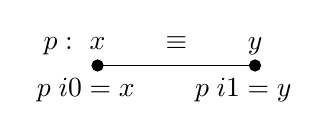
\begin{tikzpicture}
    \node [anchor=base] at (-1.5 , 0.2) {$p :$};
    \node [anchor=base] at (-1   , 0.2) {$x$};
    \node [anchor=base] at ( 0   , 0.2) {\AgdaFunction{\(\equiv\)}};
    \node [anchor=base] at ( 1   , 0.2) {$y$};
    \node [anchor=base] at (-1.15,-0.4) {$p\;\AgdaFunction{i0} = x$};
    \node [anchor=base] at ( 0.85,-0.4) {$p\;\AgdaFunction{i1} = y$};
    \draw (-1  ,0) -- ( 1,0);
    \filldraw[black] (-1,0) circle (2pt);
    \filldraw[black] (1,0) circle (2pt);
  \end{tikzpicture}
  \caption{Diagram of the Path \(p\) Between \(x\) and \(y\)}
  \label{path-diagram}
\end{marginfigure}

This is actually a perfectly usable equality type in CuTT, although the
elimination rule is a little complex and we won't look into it just yet.
However we prefer to represent equalities in a slightly more primitive way, as
it turns out to be a little more flexible.
This is the \emph{path} representation.

When represented as a path, an equality between two values of type \(A\)
actually behaves more like a function from \AgdaDatatype{I} to \(A\).
\AgdaDatatype{I} here is the type of the interval: it ranges from
\AgdaInductiveConstructor{i0} to \AgdaInductiveConstructor{i1}.
So, as a function then, when the path \(x\;\AgdaFunction{\(\equiv\)}\;y\) is
applied to \AgdaInductiveConstructor{i0}, it returns \(x\), and when it is
applied to \AgdaInductiveConstructor{i1}, it returns \(y\).

\begin{marginfigure}
  \begin{tikzpicture}
    \node [anchor=base] at (-1.8, 0.2) {$\AgdaFunction{sym}\;p :$};
    \node [anchor=base] at (-1  , 0.2) {$y$};
    \node [anchor=base] at ( 0  , 0.2) {\AgdaFunction{\(\equiv\)}};
    \node [anchor=base] at ( 1  , 0.2) {$x$};
    \node [anchor=base] at (-1.53,-1  ) {
      $\begin{aligned}
        \AgdaFunction{sym}\;p\;\AgdaFunction{i0} &= \\
        p\;(\AgdaOperator{\AgdaPrimitive{\textasciitilde{}}}\;\AgdaFunction{i0}) &= \\
        p\;\AgdaFunction{i1} &= y
      \end{aligned}$
    };
    \node [anchor=base] at ( 0.48,-1  ) {
      $\begin{aligned}
        \AgdaFunction{sym}\;p\;\AgdaFunction{i1} &= \\
        p\;(\AgdaOperator{\AgdaPrimitive{\textasciitilde{}}}\;\AgdaFunction{i1}) &= \\
        p\;\AgdaFunction{i0} &= x
      \end{aligned}$
    };
    \draw (-1  ,0) -- ( 1,0);
    \filldraw[black] (-1,0) circle (2pt);
    \filldraw[black] (1,0) circle (2pt);
  \end{tikzpicture}
  \caption{Diagram of \(\AgdaFunction{sym}\;p\)}
  \label{sym-diagram}
\end{marginfigure}

Already we can manipulate paths in some interesting ways.
First, we can manipulate values in the interval: we can take the inverse of a
point in the interval, for instance.
It's worth thinking about what this ``inverse'' corresponds to in the equality:
we will name it in the next listing.
\begin{agdalisting}
  \ExecuteMetaData[agda/Snippets/Equality.tex]{sym-def}
\end{agdalisting}
We will see some more intricate ways to manipulate paths later on, but for now
the ``function from an interval'' intuition is enough to understand the basics.

\section{Some Proofs of Equality}
So now that we know something about the equality type, let's put it to some use.
We can construct equality proofs of things which are ``obviously equal'' with
the following function:
\begin{agdalisting}
  \ExecuteMetaData[agda/Snippets/Equality.tex]{refl-def}
\end{agdalisting}
With this we can prove that the output from Equation.~\ref{example-static-eval}
is 8:
\begin{agdalisting*}
  \ExecuteMetaData[agda/Snippets/Expr.tex]{example-static-proof}
\end{agdalisting*}

Of course, these proofs aren't very interesting.
Something a little more complex might be the following:
\begin{agdalisting}
  \ExecuteMetaData[agda/Data/Nat/Properties.tex]{plus-assoc}
\end{agdalisting}
Unfortunately we can't look at much more complex proofs without building up some
more machinery around path types: we can't currently compose paths, for
instance.
\section{Quotients}
We've seen that data types can be defined by listing their constructors, where
each constructor is just a function whose return type is the type being defined.
However, we've also seen that equalities are just functions from the interval.
If we combine these two notions, we can actually define a \emph{higher
  inductive} type.
\begin{definition}[Higher Inductive Type]
  A normal inductive type (like \AgdaDatatype{Bool}, or \agdambb{N}) is a type
  where its \emph{point} constructors are listed.
  A higher inductive type can have point constructors, but it can also have
  \emph{path} constructors: instead of adding new values to the type, these
  constructors add new equalities to the type.
\end{definition}

One of the nice aspects of CuTT is that higher inductive types arise naturally
from the ``function from an interval'' interpretation of path types.
Expand out the definition of \AgdaFunction{\(\equiv\)} in the following type,
for instance:
\begin{agdalisting}
  \ExecuteMetaData[agda/Snippets/Circle.tex]{circle-def}
\end{agdalisting}
We see that the \AgdaInductiveConstructor{loop} constructor, though odd looking,
still does represent a function whose return value is
\AgdaDatatype{\(\text{S}^1\)}.

Just with regards to this \AgdaDatatype{\(\text{S}^1\)} type: it's actually the
HoTT representation of the \emph{circle}.
We won't examine its more interesting properties all that much: however it is a
good example of the simplest type with complex homotopy, so we will use it to
demonstrate several HoTT principles.

A different HIT that we \emph{will} examine in depth, however, is the following:
\begin{definition}[Set Quotient]
  In CuTT we can define the type of sets quotiented by a relation \(R\) as
  follows:
  \begin{agdalisting*}
    \ExecuteMetaData[agda/Snippets/Quotient.tex]{quot-def}
  \end{agdalisting*}
\end{definition}

So we have three constructors for our set quotient type: first, a constructor
that takes a value of the underlying type (\(A\)), and constructs a value in the
quotiented type.
Second, we see a \emph{path} constructor: this constructor does the actual
quotienting in the type.
It says that if there exists a relation \(R\) between two elements \(x\) and
\(y\) then there is also a path between the elements
\(\AgdaInductiveConstructor{\([\)}\;x\;\AgdaInductiveConstructor{\(]\)}\)
and
\(\AgdaInductiveConstructor{\([\)}\;y\;\AgdaInductiveConstructor{\(]\)}\).

The third constructor is a little bit beyond what we can explain at this point:
it \emph{truncates} the higher homotopy out of the type.
Effectively, it makes the type slightly more ``well-behaved'' with regards to
HoTT internals: without this constructor, the type would have a lot of
interesting structure which is far too interesting for us at this point.
\todo{introduce explanation now or later?}

We are going to define a type similar to the one above, but for expressions.
It will quotient out common arithmetic identities:
\begin{agdalisting}
  \ExecuteMetaData[agda/Snippets/Expr.tex]{quot-expr}
\end{agdalisting}
To evaluate this expression, we have to actually prove that the evaluation
function respects the given equality.


%%% Local Variables:
%%% mode: latex
%%% TeX-master: "../paper"
%%% End: